\documentclass{report}
% Packages
\usepackage{titlesec}
\usepackage{graphicx}
\usepackage{lipsum} % For dummy text, you can remove this
\usepackage[style=numeric, backend=biber]{biblatex} % Import the package for reading .bib files
\addbibresource{Communication.bib} % Add the .bib file
\usepackage{algorithm}
\usepackage{algpseudocode}

% Title page
\title{Dissertation Title}
\author{Luis Yallico Ylquimiche}
\date{\today}

\begin{document}

% Title page
\maketitle

% Abstract
\begin{abstract}
LOREM IPSUM
\end{abstract}

% Table of contents
\tableofcontents

% Chapters
\chapter{Introduction}
Human speech likely emerged as vital tool for coordination and the formation of social bonds among early humans [Charles Darwin's Descent of Man]. The concept, that language evolved as an adaptive trait via natural selection is widely accepted by the scientific community. 

Inspired by nature's evolutionary strategies, Swarm Engineers aspire to harness the collective intelligence mechanisms evident in social insects such as ants and bees [Ref]. This dissertation examines the communication protocols of a swarm of robots, with the aim to engineer a communication framework that enables robots to efficiently share information and collaborate on tasks, mirroring the sophisticated social interactions found in natural systems.


\section{Background}
\lipsum[1-2] % Replace with your content

\chapter{Literature Review}
\section{Previous Studies}
\lipsum[3-4] % Replace with your content

\chapter{Implementation}

Each swarm member is tasked with solving the Rastrigin function, a non-convex optimisation problem used to benchmark optimization algorithms due to its large number of local minima [REF]. THis implementation uses genetic algorithms (GA) to find the global minimum for this task. As the local population in each agent evolves, the swarm begins to communicate their current best fitness and corresponding genes to their peers. This is based on the Island model [ref], where different subpopulations (islands) evolve in parallel and occasionally exchange individuals (migration) with other islands, thus enabling the swarm to converge to a solution. Figure X, depicts the event driven one-way communication once the GA stagnates where the agent pushes its best solution to other swarm members via ESPNOW and/or via the IR board. This communication protocol was designed to avoid having to handle pull type protocols which would involve having to handle requests and responses in a sequential manner.\\  

The implementation employs an elitist immigrant-K strategy, where the best remote genes from another swarm member are integrated into the local population by replacing the worst performing K local individuals, thus preserving high-quality diversity [REF]. To counteract swarm stagnation on a local-minimum, a mass extinction event together with a hyper-mutation mechanism tracks consecutive non-improving generations. Once a set of conditions is reached (Figure X), the mutation probability is temporarily increased to escape local optima and lowest performing half of the population is re-initialised. This is done to promote exploration across the swarm and prevent premature convergence [REFS]. The swarm is considered to have completed the task, when either (i) the global minimum of 0.00 is found by at least one peer or (ii) a time limit for the task is reached.


\section{System Architecture}

Each swarm member boots into a FreeRTOS runtime by calling \texttt{app\_main()}, which performs the initialisation of the following components: non-volatile storage (NVS), I2C peripherals (APC, IR board, LVGL display, Pololu 3pi+), Real Time Clock (RTC), SD-Card, and ESPNOW. Figure X illustrates the sequence of these and their relation to the tasks that are spawned during run time. Some of these tasks include:
\begin{itemize}
  \item \texttt{gui\_task}: Manages the graphical user interface (GUI) on the M5Stack display, use for real-time feedback and debugging.
  \item \texttt{i2c\_task}: Handles communication with the I2C peripherals, including the AXP192 power supply, the IR half-duplex board, the display and the Pololu 3pi+.
  \item \texttt{ota\_task} (conditional): Manages Over-the-Air (OTA) updates if a new version is available in S3, allowing for remote software updates. Section \ref{sec:ota} has more details on this.
  \item \texttt{espnow\_task}: Manages ESPNOW communication between swarm members, handles message sending and receiving.
  \item \texttt{ga\_task}: Runs the local Genetic Algorithm (GA) for solving the Rastrigin function, coordinating with other tasks to log and transmit data.
  \item \texttt{write\_task}: Handles SD card operations, including logging data and managing file storage.
\end{itemize} 

Inter-task coordination is managed by event groups and queues, which facilitate coordinating between tasks and ensure that data is processed sequentially. The event groups are used to signal task completion and synchronise downstream operations, whereas queues are used to pass data between tasks that are operating in parallel. This enables multitasking and real-time processing of events, which differs from traditional SENSE, PLAN, ACT architectures that operate sequentially.\\

Following initialization and the conditional OTA update, each robot enters the experiment phase shown in Algorithm \ref{alg:swarm-loop}. 

Each robot is assigned a random starting point (seed) within the Rastrigin search space. The random seed is obtained via HTTPS from a server that streams quantum fluctuations in vacuum. This is to ensure that the seed is truly random and not influenced by any external factors. This initial population with its own set of random genes will thereafter undergo selection via a fitness function and genetic operators (mutation and crossover) to evolve the population.

The \texttt{ga\_task} evolves a local population until 30 generations are reached without achieving a 0.01 improvement in population fitness [REF]. At which point the best solution fitness score and genes are sent via ESPNOW to all swarm agents in a random order [NEED TO EXPLAIN WHY THIS WAS DONE]. ESPNOW send/receive callbacks measure per-packet latency (via ACKs), enqueue incoming frames to \texttt{ga\_buffer\_queue}, and count bytes for a throughput timer. The \texttt{espnow\_task} then dequeues and parses all events, updating statistics and evaluating remote genomes to \texttt{ga\_integrate\_remote\_solution}. 

\begin{algorithm}[h]
\caption{Swarm Member Experiment Loop\label{alg:swarm-loop}}
\begin{algorithmic}[1]
  \State \textbf{Init} peripherals, Wi-Fi, ESPNOW, tasks, event groups, queues
  \State Fetch quantum seed via HTTPS; \Call{init\_ga}{seed}
  \Loop
    \State \textbf{Run GA:} \Call{evolve}{}
    \State Wait until \texttt{ga\_ended} \Comment{set in \texttt{ga\_complete\_callback}}
    \State \Call{espnow\_push\_best\_solution}{local\_best}
    \State $ga\_has\_run\_before \gets \mathrm{true}$; $s\_last\_ga\_time \gets \mathrm{now}$
    \State \Call{drain\_buffered\_messages}{} \Comment{Dequeue all ESPNOW frames}
    \ForAll{msg in \texttt{ga\_buffer\_queue}}
      \State \Call{ga\_integrate\_remote\_solution}{msg.genes}
    \EndFor
    \State \Call{check\_hyper\_mutation}{} \Comment{Adjust mutation if stagnated}
    \State Reset \texttt{ga\_ended}
  \EndLoop
\end{algorithmic}
\end{algorithm}

An experiment is terminated when one of the following criteria is met:
\begin{enumerate}
  \item \textbf{Global Solution Achieved}: Any robot attains the exact global minimum of the Rastrigin function (fitness\,=\,0).
  \item \textbf{Time Limit Exceeded}: A configurable maximum duration (e.g., 10 minutes) elapses without global convergence.
\end{enumerate}
Upon termination, all ESPNOW tasks drain pending message queues, final fitness and communication metrics are written to the SD card, and log files are uploaded to an Amazon S3 bucket over HTTPS. Finally, the system de‐initializes peripherals (Wi‐Fi stopped, SD card unmounted, IR board halted) to ensure a clean shutdown.

\section{Reasons for choices}
Why use ESP-IDF over Arduino IDE in this project? \cite{esp-boards_esp-idf_nodate}\cite{expressif_freertos_nodate}

As we are using a ESP32 microcontroller to build our swarm, which left us with two options to program it: Arduino IDE or ESP-IDF. The reasons we chose the latter are because, first, it is the official development framework for the ESP32 microcontrollers, this means that ESP-IDF is native to ESP32 whereas Arduino is an API wrap around ESP-IDF. Making ESP-IDF more stable and enabling more advanced features, specially for communication data links such as Bluetooth and Wifi. Secondly, it is more powerful and flexible than Arduino IDE, because it allows the use of FreeRTOS which allows multi core development support (our M5 Stack has two cores) and is a pre-requisite for running microROS in the ESP32 microcontroller (at the time of writing this microROS does not support Arduino), hence making it more suitable for complex projects like this one. Thirdly, it is more efficient in terms of memory and speed (as it enables parallel processing) which is important for a project that requires real-time communication between multiple devices in a swarm. Finally, it is more professional and an industry standard, it allows dependency tracking, Over the Air (OTA) updates, unit testing, enhanced debugging and comprehensive documentation around it, which means it is more likely to be supported in the future and software is less likely to become deprecated over time.

How was the WIFI implementation done?

We utilized the built-in WiFi capabilities of the ESP32 with the ESPNOW communication protocol, which supports multiple unicast connections. While ESPNOW can theoretically handle around 20 devices simultaneously, practical limits are dictated by environmental factors. Additionally, ESPNOW enables multicast data transmission to multiple devices on the same channel, which can be used to pair devices or send messages to multiple swarm members. The protocol operates at a default bitrate of approximately 1 Mbps, although a portion of this bandwidth is consumed by necessary overhead, such as the MAC header. For our implementation, each swarm robot was pre-configured with the MAC addresses of all peers to facilitate direct communication. %might need to add multicast implementation
One key aspect to point out in this implementation is that connection handling and device pairing, which oversees how swarm members join and leave a connection. In its most basic form, we created a loop that goes over each MAC address and tries to rely a direct message to each other member in the swarm, to server as our benchmark. It is understood that the implications of this can have an impact on data loss and latency of the network.
For expanding a swarm dynamically, cryptographic keys might be needed to securely onboard new members, this however is out of scope of the current study.

How was the IR implementation achieved?

Using the IR board, described previously. We connected the M5Stack via the external I2C port, furthermore we had to use the Arduino library as a component of the ESP-IDF implementation for the this to work, this was due to compatibility issues between ESP-IDF and Arduino libraries. The board itself is running with an Arduino Nano to process the IR signals into messages and then sending this data accross via the SDA/SCL pins. One major implication for this, was the need to change the FreeRTOS clock speed from 100Hz to 1000Hz which improves responsiveness but at the cost of higher CPU load and power consumption. Some key parameters also include the frequency if the I2C itself which was set at 100kHtz and the master/slave configuration (M5 being the master device), this is initialized from the M5 once powered on after the 5V bus is switched on (to power the board). For more details regarding the IR board implementation please see X. 

How was the ESPNOW implementation achieved?

We used ESPNOW by pre-registering each swarm member’s MAC address, enabling unicast communication once the local GA finishes. Incoming data is placed on a queue for processing, and latency is measured via ACK callbacks. A periodic timer tracks overall throughput, logging key events as data arrives. This setup ensures efficient message handling without interfering with ongoing local genetic algorithm as it run co-curretly.


\section{OTA}\label{sec:ota}


% TODO: include references
Integrating Over-the-Air (OTA) updates into robotic swarms improves efficiency in deploying and managing software, especially in remote or hazardous environments like space or disaster zones. This scalable approach allows remote management of the entire fleet, ensuring all robots consistently run the latest software. For instance, in the automotive sector Tesla's software-enabled feature activation model showcases how OTA updates can enhance customer services and streamline hardware production by allowing quick, widespread deployment of critical updates.

Using cloud services like AWS S3 for hosting OTA updates ensures high availability and safe rollback capabilities in our system, increasing robustness against failures like incomplete updates due to power loss. This setup reduces capital expenditure costs and improves swarm scalability compared to local servers that can become a single source of failure. Mirroring Apple’s use of cloud infrastructure for massive, global iOS updates—but also complies with regional data laws by using decentralized storage and managed encryption.

Our project integrates Continuous Integration and Deployment (CI/CD) to maintain dynamic software development for the swarm. This ensures that features and fixes are promptly integrated and tested, maintaining software quality and allowing the swarm to consistently operate with the latest releases. This approach is crucial for testing various communication parameters within our experiments, ensuring reliable and systematic updates.

\begin{figure}[h]
    \centering
    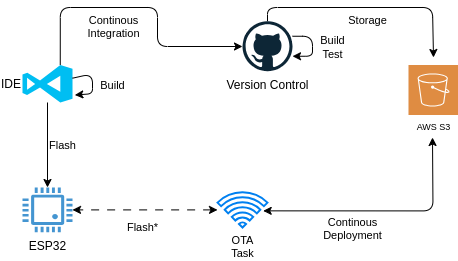
\includegraphics[width=0.5\textwidth]{architecture.png}
    \caption{System Architecture}
    \label{fig:architecture}
\end{figure}

Figure \ref{fig:architecture} shows the implementation of our system to enable over the air updates (OTA) and continuous integration \& continuous deployment (CI/CD) framework over the swarm. 
\begin{itemize}
    \item \textbf{Local Development Environment}: ESP32 application development takes place locally using VSCode, the IDE environment uses version 5.2.2 of ESP-IDF and Python 3.11 to build and flash the code in-situ to the ESP32 module. This self contained development environment allows for testing new features and updates without affecting previous versions of the application running on the swarm.
    \item \textbf{Version Control System \& CI/CD}: The codebase is stored in a public repository on GitHub: \url{https://github.com/yallico/robotics_dissertation}, this allows for version control and automates the build and test process upon every commit. The ESP32 project is compiled and it generates the .bin binary file used for OTA. This process ensures that the codebase is always in a working state and ready for deployment.
    \item \textbf{Cloud Storage}: Once the OTA binary file is generated, it is uploaded to an AWS S3 public bucket. S3 serves as a reliable and low cost storage solution for the OTA updates. We decided to leave encryption and access control out of scope from the OTA implementation, yet we acknowledge that encryption is a non-trivial task that swarms should consider when deploying OTA updates in terms of computational resources required and security implications in industry. %TODO: Add reference to encryption in OTA
    \item \textbf{OTA Update Process}: The ESP32, runs a task that is triggered upon initialisation which compares its current application version against the latest version available in S3. If the version in AWS S3 diverges from the current version running in the ESP32. It then downloads the .bin file and performs the update following OTA best practice (see Section X). %TODO: Add reference to OTA best guidance from ESP-IDF.

\end{itemize}

\section{Data Capture}
We implemented local data logging on the M5Stack by integrating a 16GB SD card peripheral, using the SPI bus (shared by the LCD) set at a frequency of 20MHz and utilizing the FAT32 file system for storage. This approach was chosen to emulate a realistic swarm system capable of operating remotely without relying on a stable Wi-Fi connection to a central server. Local logging minimizes data transmission loss, supporting the swarm's objective of avoiding any single point of failure. 

Upon completing the experimental tasks, the swarm members switch to a data upload mode, where the locally collected data is securely transmitted to an S3 bucket using HTTPS. This might seem counter intuitive to our original decentralized objective, but it was planned to be this way as otherwise we would have to manually read each individual SD card to collect the data, which would be time consuming and error prone. Furthermore, we expect that in a real world scenario, the swarm would be deployed in a remote location where manual data collection would be impossible.

Data logs are saved in the root directory of the SD card in a \.json format. Our system is designed to automatically generate new files upon reaching a specified size limit, this enables efficient memory management and preventing heap memory overflow during log file writes.


\newpage
\section{Preliminary Sensitivity Analysis}

\begin{figure}[h]
    \centering
    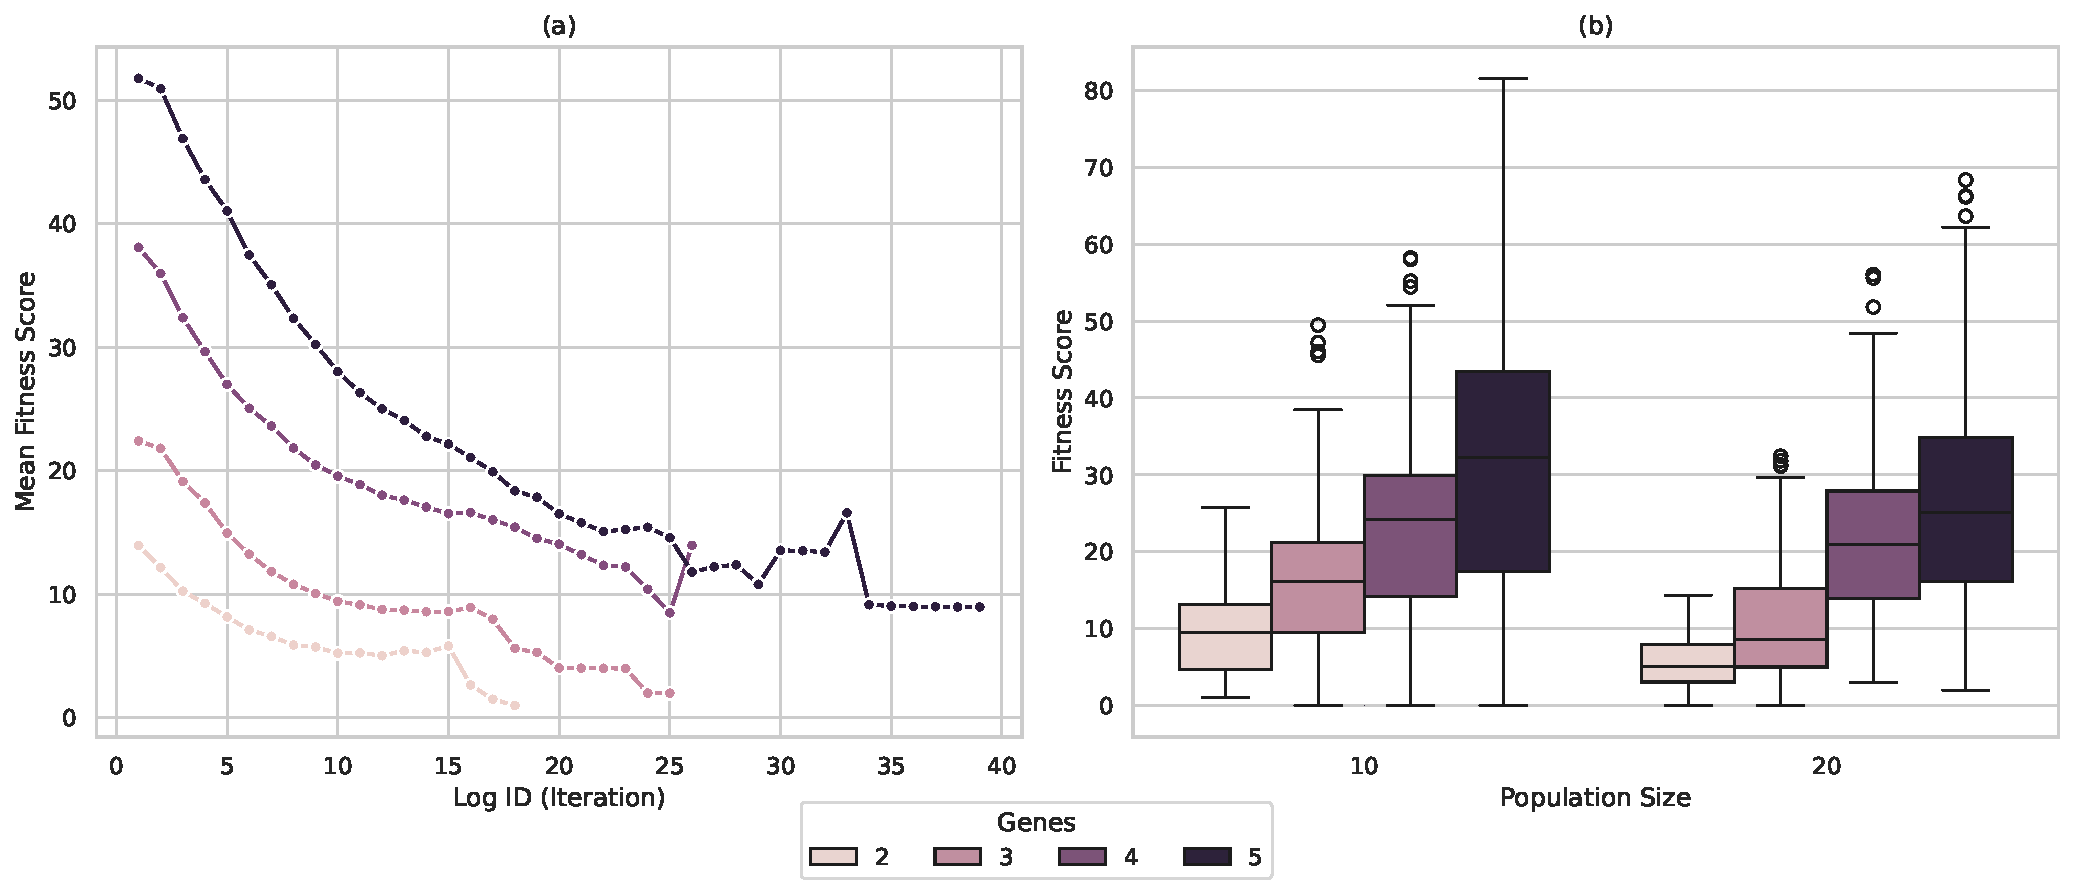
\includegraphics[width=1\textwidth]{ga_prelim_analysis.pdf}
    \caption{a: Number of iterations for algorithm to converge to either a global or local minimum. b: Fitness distribution by population size and genes.}
    \label{fig:ga_prelim_analysis}
\end{figure}

Using a single robot, a preliminary analysis was conducted to identify suitable parameters for solving the Rastrigin function under varying population sizes and gene dimensions. A total of \textbf{136 experiments} were performed, each terminating if fitness failed to improve beyond a \textbf{0.001 threshold} over \textbf{20 consecutive epochs} (patience). %TODO: Include reference for the patience parameter
Only iterations exceeding this improvement threshold were logged. If the global optimum (fitness=0) was not reached, the run was considered converged to a local minimum. Across all runs, convergence times ranged \textbf{from 0 to 3 seconds}, reflecting the early stopping triggered by the patience setting. As shown in Figure~\ref{fig:ga_prelim_analysis}, larger populations and higher iteration counts generally yielded lower final fitness, consistent with the genetic algorithm’s search properties.\\

A practical takeaway from the data is that using five genes is sufficiently challenging to extend the runtime into the range of minutes rather than seconds, even though a single robot with fewer genes can solve the function in only a couple of seconds. This configuration will ensure that experiments in a swarm environment will involve cooperation, where the exchange of best solutions between members could permit convergence for a five-dimensional Rastrigin function.






% Add more chapters as needed

\newpage
\printbibliography

\end{document}